\documentclass[a4paper,11pt]{article}
\input{/home/tof/Documents/Cozy/latex-include/preambule_lua.tex}
\newcommand{\showprof}{show them}  % comment this line if you don't want to see todo environment
\fancyhead[L]{Architecture de von Neumann}
\newdate{madate}{03}{09}{2020}
\fancyhead[R]{Première - NSI} %\today
\fancyfoot[L]{~\\Christophe Viroulaud}
\fancyfoot[C]{\textbf{Page \thepage}}
\fancyfoot[R]{\includegraphics[width=2cm,align=t]{/home/tof/Documents/Cozy/latex-include/cc.png}}

\begin{document}
\begin{Form}
\begin{commentprof}
\paragraph{devoir:} Construire ce cours sous forme de carte mentale.
\end{commentprof}
\paragraph{Objectif:}Distinguer les constituants d'une machine et leur rôle.

\section{Problématique: comment ça fonctionne?}
Une tablette, un smartphone, un ordinateur portable sont des objets du quotidien. Il s'agit d'objets qui reposent tous sur le même principe: l'ordinateur.
\begin{figure}[!h]
\centering
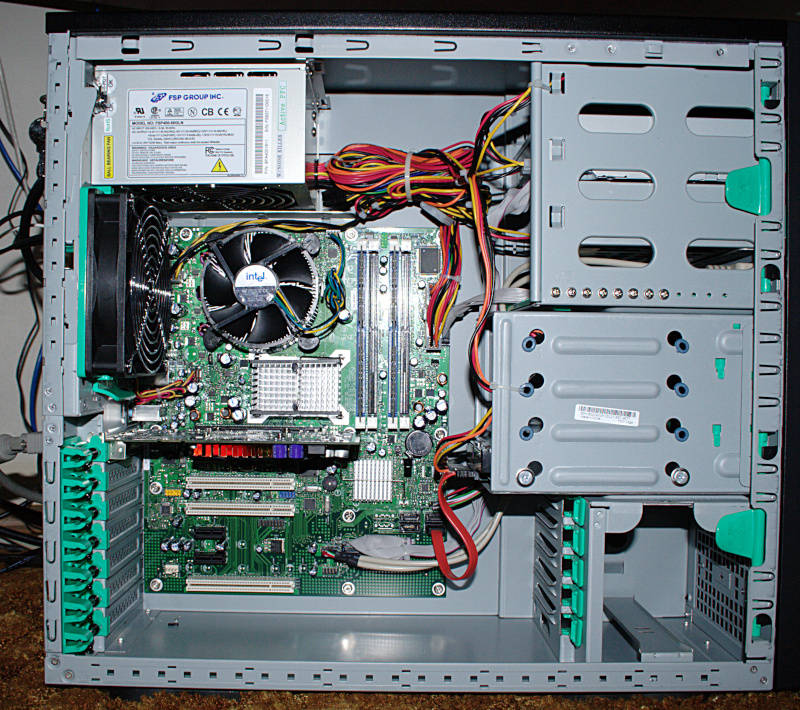
\includegraphics[width=7cm]{ressources/inside-pc.jpg}
\captionof{figure}{à l'intérieur d'un ordinateur}
\label{inside}
\end{figure}
\begin{center}
\shadowbox{\parbox{14cm}{\centering Quels sont les concepts qui régissent le fonctionnement d'un ordinateur?}}
\end{center}
\section{Composants d'un ordinateur}
Quand on ouvre un ordinateur, nous pouvons distinguer plusieurs types de composants:
\begin{itemize}
\item \emph{Unité de calculs}: le processeur ou CPU (Control Processing Unit) sous le ventilateur,
\item \emph{Mémoire}: composée d'une ou plusieurs barrettes,
\item \emph{Périphériques d'entrée-sortie}: permettent une interaction avec l'ordinateur; en entrée, en sortie ou les 2 (disque dur, clavier, imprimante...).
\end{itemize}
D'autres composants ne sont pas détaillés ici:
\begin{itemize}
\item carte graphique: processeur spécialisé,
\item alimentation,
\item carte-mère: met en relation les composants.
\end{itemize}
\section*{Retour historique}
\begin{itemize}
\item Atanasoff / Mauchly, Eckert = procès; on a reconnu la paternité des idées à Atanasoff.
\item Mark I est utilisé pour déchiffrer le code de Lorenz employé par les Allemands; constitué de 1500, puis 2400 tubes à vide.
\item Plus rapide, le Colossus Mark II servit notamment pour le lancement surprise du Débarquement.
\item ENIAC acronyme de Electronic Numerical Integrator And Computer, servait à effectuer calculs balistiques. Il peut être reprogrammé pour résoudre, en principe, tous les problèmes calculatoires. Mauchly = idée; Eckert = ingénierie notamment durée de vie des tubes électroniques (tubes à vide); Z3 encore électromécanique.
\item transistor: gagne en fiabilité; commence à le fabriquer à faible coût dès 1950; début miniaturisation. chercheurs des laboratoires BEll. Aujourd'hui les circuits intégrés contiennent des millions de transistors
\item EDVAC (Electronic Discrete Variable Automatic Computer) Mauckly, Eckbert et Neumann à la manœuvre. Il opère en mode binaire contrairement à l'ENIAC, qui opère en décimal.
\item 2019: aujourd'hui on ne soude plus les transistors "à la main"; circuit intégré: dépôt de différentes couches de matériaux; finesse de gravure.
\end{itemize}
\section{Le modèle de von Neumann}
John von Neuman est introduit dans le projet ENIAC en 1944. L'idée principale de son rapport est de faire que le programme soit enregistré dans la mémoire. Il ne sera donc plus nécessaire de changer le câblage du calculateur pour chaque changement de programme.\\
L'ordinateur contemporain reprend l'architecture édictée par John von Neumann en 1945.
\begin{figure}[!h]
\centering
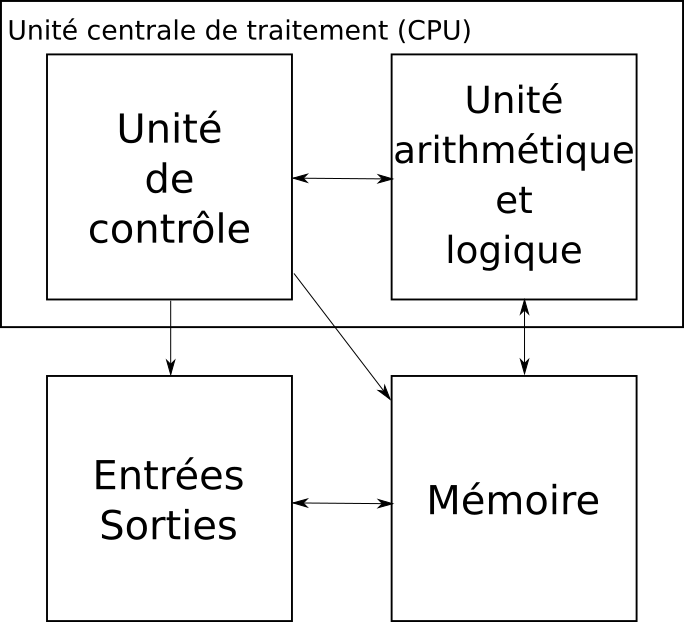
\includegraphics[width=7cm]{ressources/von-neumann.png}
\captionof{figure}{Architecture de von Neumann}
\label{neumann}
\end{figure}
\subsection{CPU}
\subsubsection{Unité Arithmétique et Logique}
effectue opérations arithmétiques et opérations sur les \emph{bits}. Composée de plusieurs registres:
\begin{itemize}
\item \emph{Registres de données}: stocke données en cours d'utilisation,
\item \emph{Accumulateur}: effectue les calculs
\item \emph{circuits électroniques}: opérations arithmétiques (addition...), logiques (et, ou...), comparaisons.
\end{itemize}
Différents types de registres spécialisés comme \emph{le compteur ordinal}: indique l'emplacement de la prochaine instruction à être exécutée (synonymes : compteur de programme, pointeur d'instruction).
\subsubsection{Unité de Contrôle}
chef d'orchestre de l'ordinateur. Elle doit:
\begin{itemize}
\item lire le programme,
\item décoder les instructions,
\item commander leur exécution (par l'UAL).
\end{itemize} 
\subsection{Mémoire}
\subsection{Organisation de la mémoire}
Une mémoire est un circuit à semi-conducteur permettant d’enregistrer, de conserver et de restituer des
informations (instructions et variables). C’est cette capacité de mémorisation qui explique la polyvalence
des systèmes numériques et leur adaptabilité à de nombreuses situations. Les informations peuvent être
écrites ou lues.
\subsubsection{Mémoire vive ou volatile}
Elle contient à la fois les données et le programme qui indiquera à l’unité de contrôle quels sont les calculs à faire sur ces données. Les données stockées peuvent être lues, effacées, déplacées. Rapidité d'accès. Perd son contenu dès qu'on éteint l'ordinateur. On parle souvent de RAM (Random Access Memory).
\subsubsection{Mémoire non volatile}
Conserve ses données à l'extinction. Exemple: mémoire ROM (Read Only Memory) qui contient données nécessaires au démarrage de l'ordinateur.
\subsection{Entrées-Sorties}
\subsubsection{Entrées}
\begin{itemize}
\item claviers, souris,
\item manettes, lecteurs code-barres,
\item scanners, webcams.
\end{itemize}
\subsubsection{Sorties}
\begin{itemize}
\item écrans,
\item imprimantes,
\item haut-parleurs.
\end{itemize}
\subsubsection{Entrée et Sortie}
\begin{itemize}
\item lecteurs de disques,
\item disques durs, clé USB,
\item carte réseau.
\end{itemize}
\subsection{Transmission des données}
Les \emph{bus} sont les liaisons très rapides qui permettent aux bits de circuler. Le terme dérive du latin omnibus (à tous). En pratique, des câbles.
\section{Évolution}
\begin{itemize}
\item Les entrées-sorties, initialement commandées par l’unité centrale, sont depuis le début des années 1960 sous le contrôle de processeurs autonomes; mise en place utilisation en temps partagé.
\item Les ordinateurs comportent maintenant des processeurs multiples; gain rapidité de calculs.
\end{itemize}
Ces deux évolutions ont pour conséquence de mettre la mémoire, plutôt que l’unité centrale, au centre de
l’ordinateur, et d’augmenter le degré de parallélisme dans le traitement et la circulation de l’information.
Mais elles ne remettent pas en cause les principes de base que sont la séparation entre traitement et
commande et la notion de programme enregistré.
\section{Limites du modèle}
\subsection{Temps d'accès}
Ce modèle impose un va-et-vient constant entre CPU et mémoire. Cependant la différence entre vitesse des microprocesseurs (nombre d'opérations par seconde) et mémoire (temps d'accès) est très importante. Les CPU passeraient la majorité de leur temps à attendre. Un processeur cadencé à 3GHz effectue $3.10^9$ opérations par seconde. C'est \emph{le goulot d'étranglement} du modèle de von Neumann.\\Les fabricants ont inventés des \emph{mémoires caches} situées proches du CPU. L'idée principale est qu'une donnée utilisée une fois a de grandes chances d'être utilisée plusieurs fois.
\subsection{Hiérarchie des mémoires}
\begin{tabular}{|*{2}{>{\centering\arraybackslash}m{.4\textwidth}|}}
\hline 
Mémoire & Temps d'accès \\ 
\hline 
registres & 1ns \\ 
\hline 
mémoire cache & 2-3ns \\
\hline
mémoire vive & 5-60ns \\
\hline
disques durs & 3-20ms \\
\hline
DVD & 140ms \\
\hline
\end{tabular} 
\end{Form}
\end{document}